%%%%%%%%%%%%%%%%%%%%%%%%
%
% $Author: Sadegh Naderi $
% $Datum: 2023-07-01  $
% $Pfad: BA23-02-Sales-Predictor/report/Contents/en/Packages.tex $
% $Version: 1.0 $
% $Reviewed by: Deepti, Sadegh and Raunak $
% $Review Date: 2023-07-02 $
%
%%%%%%%%%%%%%%%%%%%%%%%%




\chapter{Development Environment}

\section{Introduction}

A development environment refers to the integrated set of tools, software, and resources that facilitate the creation, testing, and deployment of software applications. It provides developers with a structured and efficient workflow, enabling them to write, edit, and debug code while ensuring compatibility and efficiency. Development environments typically include code editors, compilers or interpreters, debuggers, version control systems, and other utilities tailored to the specific programming languages or frameworks used. They aim to streamline the development process, enhance collaboration, and improve productivity by offering features such as code autocompletion, syntax highlighting, code refactoring, and seamless integration with other development tools and services.

\section{What it is used for}

A development environment is primarily used by software developers to create, modify, and maintain software applications. It serves as a centralized workspace where developers can write and edit code, compile or interpret it into executable form, debug and test their applications, and manage their projects. The development environment provides a range of tools and features that streamline the development process, such as code completion, syntax highlighting, error checking, and version control integration. It also allows for efficient collaboration among developers, enabling them to work on the same codebase, share and review code, and track changes. Ultimately, a development environment enhances productivity, facilitates efficient coding practices, and supports the creation of high quality software applications.

\section{versions}

\begin{enumerate}
	\item Programming Language: Python (\textbf{version: 3.10.11})
	\begin{itemize}
		\item The code is written in Python, a widely used programming language for data analysis and machine learning tasks.
	\end{itemize}
	\item Libraries and Packages:
	\begin{itemize}
		\item pandas (\textbf{version: 2.0.2}): Used for data manipulation and analysis. It provides data structures and functions to efficiently handle structured data.
		\item numpy (\textbf{version: 1.25.0}): Used for numerical computations and operations on arrays. It provides efficient mathematical functions for working with arrays.
		\item matplotlib (\textbf{version: 3.7.1}): Used for data visualization. It provides functions to create various types of plots and charts.
		\item datetime: Used for manipulating dates and times.
		\item xgboost (\textbf{version: 1.7.6}): A popular machine learning library used for gradient boosting. It provides an implementation of the XGBoost algorithm for regression and classification tasks.
		\item scikit-learn (\textbf{version: 1.2.2}): A comprehensive machine learning library that provides various tools and algorithms for data preprocessing, model selection, and evaluation.
	\end{itemize}
	\item Conda (\textbf{version: 23.3.1)}:
	\begin{itemize}
		\item Conda is an open-source package and environment management system for Python. It simplifies installing, managing, and updating software packages and dependencies.
	\end{itemize}
	\item Data Files:
	\begin{itemize}
		\item The code reads data from several CSV files located in the 'Data' directory. These files include \textbf{'stores.csv', 'items.csv', 'transactions.csv', 'oil.csv', 'holidays\_events.csv', and 'train.csv'} .
	\end{itemize}
\end{enumerate}

It's important to note that the code assumes the availability of the required libraries, the proper installation of Python, and the presence of the data files in the specified directory. 


\section{Description}

A \textbf{conda environment} refers to a directory housing a distinct set of conda packages that have been installed. For instance, you might have an environment with NumPy 1.7 and its associated dependencies, while another environment retains NumPy 1.6 for legacy testing purposes. Modifying one environment does not impact the others, ensuring separation. Switching between environments is made simple by activating or deactivating them. Furthermore, sharing your environment involves providing a copy of your environment.yaml file to others \cite{Conda-environments:2023}.

\textbf{Why a Conda Environment is chosen:}

the main differences between a conda environment and the default environment lie in their package management and isolation capabilities. Conda environments provide a comprehensive package management system, allowing easy installation, update, and removal of packages while handling dependencies and ensuring compatibility. They offer isolation by creating separate environments with their own package sets, enabling conflict-free work on different projects. Conda environments also ensure cross-platform compatibility, allowing consistent behavior across different operating systems. In contrast, the default environment typically has limited package management capabilities and less isolation, potentially leading to conflicts and platform dependencies. 

\subsection{Main Functions}

\begin{enumerate}
	\item \textbf{Environment Creation:} The primary function of Conda is to create isolated environments. Each environment can have its own Python version and packages, independent of the system's default Python installation. This allows you to work on multiple projects with different requirements without conflicts.
	
	\item \textbf{Package Management:} Conda provides robust package management capabilities. It allows you to install, update, and remove packages within an environment. You can specify the exact versions of packages or let Conda handle the dependencies automatically.
	
	\item \textbf{Environment Activation/Deactivation:} Conda allows you to activate and deactivate environments. Activation sets the environment variables and modifies the system's PATH to use the packages installed within the active environment. This ensures that the correct Python interpreter and packages are used when running commands or scripts.
	
	\item \textbf{Environment Sharing and Replication:} Conda environments can be exported and shared with others. This allows collaborators or other users to recreate the same environment with the exact set of dependencies needed for a project. It ensures that everyone is using the same versions of packages, reducing compatibility issues.
\end{enumerate}

\subsection{Subfunctions}

\begin{enumerate}
	\item \textbf{Create an Environment:} You can create a new Conda environment using the \texttt{conda create} command. For example:
	\[
	\texttt{conda create --name myenv}
	\]
	
	\item \textbf{Activate an Environment:} To activate an environment, you can use the \texttt{conda activate} command. For example:
	\[
	\texttt{conda activate myenv}
	\]
	
	\item \textbf{Deactivate an Environment:} To deactivate an environment, you can use the \texttt{conda deactivate} command. For example:
	\[
	\texttt{conda deactivate}
	\]
	
	\item \textbf{Install Packages:} You can install packages into an environment using the \texttt{conda install} command. For example:
	\[
	\texttt{conda install numpy}
	\]
	
	\item \textbf{Update Packages:} You can update packages within an environment using the \texttt{conda update} command. For example:
	\[
	\texttt{conda update numpy}
	\]
	
	\item \textbf{Remove Packages:} To remove packages from an environment, you can use the \texttt{conda remove} command. For example:
	\[
	\texttt{conda remove numpy}
	\]
	
	\item \textbf{Export an Environment:} You can export an environment to a YAML file using the \texttt{conda env export} command. For example:
	\[
	\texttt{conda env export --name myenv --file environment.yml}
	\]
	
	\item \textbf{Create an Environment from a YAML file:} You can create an environment from a YAML file using the \texttt{conda env create} command. For example:
	\[
	\texttt{conda env create --file environment.yml}
	\]
\end{enumerate}

These are some of the main functions and subfunctions of a Conda environment. Using these commands and capabilities, you can effectively manage your Python packages and create reproducible environments for your projects.

\section{Installation}


\begin{enumerate}
	\item \textbf{Download Anaconda}: Visit the Anaconda website (\texttt{https://www.anaconda.com/products/individual}) and download the appropriate version of Anaconda for your operating system (Windows, macOS, or Linux). Choose the Python 3.x version, as it is the most recent stable release.
	
	\item \textbf{Run the Installer}: Once the Anaconda installer is downloaded, locate the file and run it. Follow the on-screen instructions to install Anaconda on your system. Choose the default installation options unless you have specific preferences.
	
	\item \textbf{Open Anaconda Prompt}: After installation, open the Anaconda Prompt. On Windows, you can find it by searching for "Anaconda Prompt" in the Start menu. On macOS and Linux, you can open a terminal window and activate the conda base environment.
	
	\item \textbf{Create a New Environment}: To create a new conda environment, use the following command:
	
	\begin{verbatim}
		conda create --name SalesPrediction
	\end{verbatim}
	
	You can choose any name you like by replacing \texttt{SalesPrediction} with the desired name for your environment. .
	
	\item \textbf{Activate the Environment}: Once the environment is created, activate it using the following command:
	
	\begin{verbatim}
		conda activate SalesPrediction
	\end{verbatim}
	
	
	\item \textbf{Install Packages}: With the environment activated, you can now install packages into it. For example, to install the  named \texttt{numpy} package, use the following command:
	
	\begin{verbatim}
		conda install numpy
	\end{verbatim}
	
	Replace \texttt{numpy} with the name of the package you want to install. You can install multiple packages in one command by separating them with spaces.
	
	In our case, these packages should be installed:
	
	\begin{verbatim}
		conda install pandas
		conda install matplotlib
		conda install xgboost
		conda install sklearn
		conda install scikit-learn
	\end{verbatim}
	
	Note the with installing the \texttt{pandas} package, the \texttt{numpy} would be automatically istalled as it is a dependency of the \texttt{pandas} package.
	
	\item \textbf{Manage Packages}: You can update packages in your environment using the \texttt{conda update} command. For example, to update \texttt{numpy}, use:
	
	\begin{verbatim}
		conda update numpy
	\end{verbatim}
	
	To remove a package, use the \texttt{conda remove} command. For example, to remove \texttt{numpy}, use:
	
	\begin{verbatim}
		conda remove numpy
	\end{verbatim}
	
	\item \textbf{Deactivate the Environment}: When you're done working in the environment, you can deactivate it using the following command:
	
	\begin{verbatim}
		conda deactivate
	\end{verbatim}
	
	This will return you to the base conda environment.
\end{enumerate}

Congratulations! You have successfully installed and created a conda environment. You can create additional environments and repeat the steps above to manage and work with different sets of packages as per your project requirements.

\subsection{Configuration}

\subsubsection{Configure using PyCharm (special Case)}

Here, the Configuration of the Python Interpreter in PyCharm to use your Conda environment is explained.

\begin{enumerate}
	\item In the settings/preferences window, navigate to the "Project" settings and select your project from the list.
	
	\item Under the project settings, locate the "Python Interpreter" option and click on it.
	
	\item In the Python Interpreter settings, click on the gear icon and select "Add..."
	
	\item In the "Add Python Interpreter" dialog, choose the "Conda Environment" option and select the "Existing environment" radio button.
	
	\item Click on the "..." button next to the "Interpreter" field and browse to the location of your Conda environment. The Conda environments are usually stored in a directory named "envs" inside your Anaconda or Miniconda installation directory.
	
	\item Once you have selected the interpreter from the Conda environment, click on the "OK" button.
	
	\item PyCharm will now set up the interpreter and show it in the list of available interpreters. Click "OK" again to save the changes and close the settings/preferences window.
	
	\item Now, when you work on your project in PyCharm, it will use the selected Conda environment as the interpreter. You can install additional packages, run your code, and access all the functionalities provided by the Conda environment.
\end{enumerate}

By configuring the Python Interpreter in PyCharm to use your Conda environment, you ensure that PyCharm uses the correct Python interpreter and the packages installed within that environment.

\subsubsection{Share the environment for other team members (general Case)}

Once you have created your conda environment, you can produce a YAML file that captures the environment's configuration. This YAML file can then be used to recreate the environment on another system or share it with others. 

Thr YAML file defines the dependencies and configurations of the Conda environment, including the required packages and their versions. It can be used to recreate the same environment on another system.

Here's how you can produce the YAML file and configure an environment based on it:

\textbf{1. Generating the YAML file:}
\begin{itemize}
	\item Open your terminal or command prompt.
	\item Activate the conda environment you want to capture using the command: \texttt{conda activate <environment\_name>}.
	\item Use the following command to generate the YAML file: \texttt{conda env export > environment.yaml}.
	\item This command exports the environment's configuration, including package names and versions, into a file named \texttt{environment.yaml}. You can choose a different name if desired.
\end{itemize}

\textbf{2. Configuring an environment using the YAML file:}
\begin{itemize}
	\item To create a new environment based on the YAML file, make sure you have conda installed and open your terminal or command prompt.
	\item Navigate to the directory where the \texttt{environment.yaml} file is located.
	\item Run the following command to create the environment: \texttt{conda env create -f environment.yaml}.
	\item Conda will read the YAML file and create a new environment with the same package configuration.
\end{itemize}

Note: The \texttt{environment\_name} in the YAML file will be the name of the newly created environment. If you want to specify a different name, you can modify the \texttt{name} field in the YAML file before running the \texttt{conda env create} command.


\subsubsection{what is more special?}

\begin{itemize}
	\item The datasets \textbf{'stores.csv', 'items.csv', 'transactions.csv', 'oil.csv', 'holidays\_events.csv', and 'train.csv'} should be in a directory named \texttt{Data}. 
	\item Users should also create a folder called \texttt{Figure\_Output} so that the extracted figure could be exported there. Due to the possibiliy of missing the data which is already in that folder, automation of creating this folder with python code is disregarded.
	\item Mac and Windows users should be aware of the differences of these operationg systems while working with Python:
	\begin{enumerate}
		\item \textbf{File Paths}: The format of file paths can differ between Mac and Windows. Windows typically uses backslashes (\textbackslash) to separate directories in a file path (e.g., "C:\textbackslash Program Files\textbackslash MyFile.txt"), while Mac uses forward slashes (/) (e.g., "/Users/Username/Documents/MyFile.txt"). When dealing with file paths in your Python code, it's important to use the appropriate path separators based on the target platform.
		
		\item \textbf{Line Endings}: Windows and Mac use different characters to represent line endings in text files. Windows uses a combination of carriage return (\textbackslash r) and line feed (\textbackslash n) characters ("\textbackslash r\textbackslash n"), whereas Mac uses only the line feed character ("\textbackslash n"). While this distinction is usually handled automatically by text editors and programming environments, it can occasionally cause issues when working with files that have been created on a different platform.
		
		\item \textbf{Platform-Specific Libraries}: Some Python libraries may have platform-specific functionality or dependencies. For example, libraries that interact with the underlying operating system, such as accessing specific system resources or executing shell commands, may require different code or have different behavior on Mac and Windows. It's important to consult the documentation of such libraries to understand any platform-specific considerations.
		
		\item \textbf{Case Sensitivity}: Mac is a case-sensitive file system by default, whereas Windows is case-insensitive. This can impact the behavior of Python code that relies on file names or other identifiers being matched exactly. It's essential to be consistent with casing when referencing files or variables to ensure cross-platform compatibility.
	\end{enumerate}
\end{itemize}


\section{First steps}



\section{Program "Hello World"}
This section provides an example program or code snippet to demonstrate the basic functionality of the development environment.

\subsection{Description}
The "Hello World" program is a simple introductory program that outputs the phrase "Hello, World!" It serves as a starting point to verify that the development environment is correctly set up and can execute code.


\subsection{Example manual: Creation and Use of Conda Environments}

1. Create a Conda environment using Anaconda Prompt on your system:

\begin{verbatim}
	conda create --name hello_env python=3.9
\end{verbatim}

when asked "Proceed ([y]/n)?" press y

This command creates a new Conda environment named "hello\_env" and specifies Python version 3.9.

2. Activate the Conda environment:

\begin{verbatim}
	conda activate hello_env
\end{verbatim}

This command activates the "hello\_env" environment, indicating that we want to use this environment for our Python code.

3. Create a Python file named \texttt{HelloWorld.py} and open it in a text editor. Add the following code:

\begin{lstlisting}[language=Python]
	## @mainpage Hello World Example
	#
	# @section author Author:
	#
	# Sadegh Naderi
	#
	#
	# @section intro_sec Introduction
	#
	# This is an example of a simple Hello World syntax created for explaining how to create a simple virtual environment.
	#
	# refer to the chapter Environment in the report for more info
	#
	# @section manual Example manual: Creation and Use of Conda Environments
	#
	# 1. Create a Conda environment using Anaconda Prompt on your system:
	# @code
	# conda create --name hello_env python=3.9
	# @endcode
	# When asked "Proceed ([y]/n)?", press 'y'.
	# This command creates a new Conda environment named "hello_env" and specifies Python version 3.9.
	#
	# 2. Activate the Conda environment:
	# @code
	# conda activate hello_env
	# @endcode
	# This command activates the "hello_env" environment, indicating that we want to use this environment for our Python code.
	#
	# 3. Create a Python file named HelloWorld.py and open it in a text editor. Add the following code:
	# @code
	# def say_hello():
	#
	#     print("Hello, World!")
	#
	# def main():
	#
	#     say_hello()
	#
	# # Call the main function to start the program
	# if __name__ == "__main__":
	#     main()
	# @endcode
	# This code defines a function say_hello() that prints the "Hello, World!" message to the console.
	#
	# 4. Save the HelloWorld.py file and close the text editor.
	#
	# 5. If needed, navigate to the directory where your Python file is located using the cd command. Execute the Python code:
	# @code
	# python HelloWorld.py
	# @endcode
	# This command runs the HelloWorld.py script using the Python interpreter in the activated Conda environment.
	# You should see the output "Hello, World!" printed to the console, indicating that the code executed successfully.
	#
	# 6. Deactivate the Conda environment:
	# @code
	# conda deactivate
	# @endcode
	# This command deactivates the current Conda environment.
	# The Anaconda Prompt should look like Figure 1.
	#
	# By following these steps, you've created a Conda environment, activated it, written a simple "Hello World" Python code, and executed it within the Conda environment. Conda allows you to manage different environments for different projects, providing isolation and dependency management for your Python applications.
	
	## @file say_hello.py
	#  @brief A simple "Hello World" program in Python.
	#
	#  This program prints the message "Hello, World!" to the console.
	
	def say_hello():
	"""! Prints the message "Hello, World!" to the console.
	@brief Processes This function prints the message "Hello, World!" to the console.
	It does not accept any arguments or return any value.
	@return None
	@see say_hello()
	"""
	
	print("Hello, World!")
	
	def main():
	"""! The main function of the program.
	@brief Processes This function is the entry point of the program. It calls the say_hello() function to print the
	"Hello, World!" message.
	@return None
	@see say_hello()
	"""
	say_hello()
	
	# Call the main function to start the program
	if __name__ == "__main__":
	main()lo() function to print the message.
	say_hello()
\end{lstlisting}

This code defines a function \texttt{say\_hello()} that prints the "Hello, World!" message to the console.


4. Save the \texttt{HelloWorld.py} file and close the text editor.

5. If needed, navigate to the directory where your Python file is located using the \texttt{cd} command. Execute the Python code:

\begin{verbatim}
	python HelloWorld.py
\end{verbatim}

This command runs the \texttt{HelloWorld.py} script using the Python interpreter in the activated Conda environment.

You should see the output \texttt{Hello, World!} printed to the console, indicating that the code executed successfully.

6. Deactivate the Conda environment:

\begin{verbatim}
	conda deactivate
\end{verbatim}

This command deactivates the current Conda environment.

The Anaconda Prompt should look like Figure \ref{rompt}.

\begin{center}
	\begin{figure}[h!]
		\begin{center}
			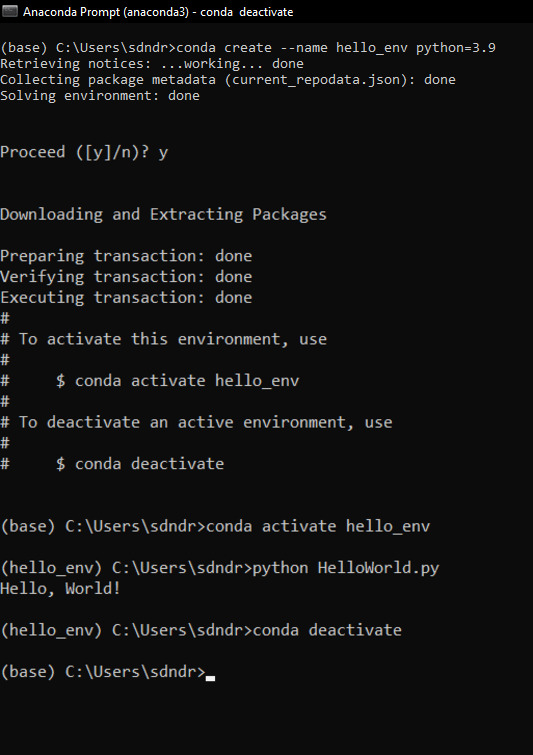
\includegraphics[height=120mm]{Images/CondaPrompt.jpg}
		\end{center}
		\caption{Creating a conda environment for HelloWorld code with Anaconda Prompt}
		\label{CondaPrompt}
	\end{figure}
\end{center}

By following these steps, you've created a Conda environment, activated it, written a simple "Hello World" Python code, and executed it within the Conda environment. Conda allows you to manage different environments for different projects, providing isolation and dependency management for your Python applications.





	
